% fig_pi_section_circuit.tex
% Pi-section line model for 87L differential relay
% Shows: local IED (S), remote IED (R), series Z, shunt Y/2 at each end,
%        fault point F at location x from S, differential measurement.
\begin{tikzpicture}[
  bus/.style  = {draw, fill=gray!15, minimum width=4pt, minimum height=32pt},
  ied/.style  = {draw, rounded corners=2pt, fill=blue!8,
                 minimum width=28pt, minimum height=18pt, font=\scriptsize},
  label/.style = {font=\scriptsize},
  conn/.style  = {draw, thick},
  shunt/.style = {draw, blue!60!black, thick},
  fault/.style = {draw, red!70!black, very thick},
  ]

  % ---- Coordinates -------------------------------------------------------
  \coordinate (S)  at (0, 0);          % sending-end bus
  \coordinate (R)  at (8, 0);          % receiving-end bus
  \coordinate (ms) at (0.8, 0);        % series line start
  \coordinate (mr) at (7.2, 0);        % series line end
  \coordinate (Fc) at (4.0, 0);        % fault point

  % ---- Bus bars ----------------------------------------------------------
  \draw[conn, line width=2pt] (S)  ++(-0.05,0.45) -- ++(0,-0.9);
  \draw[conn, line width=2pt] (R)  ++(-0.05,0.45) -- ++(0,-0.9);

  % ---- Series impedance R + jX ------------------------------------------
  \draw[conn] (ms) -- (2.8, 0);
  % Fault gap
  \draw[conn] (2.8,0) -- (3.6, 0);
  \draw[conn] (4.4, 0) -- (5.2, 0);
  \draw[conn] (5.2, 0) -- (mr);
  % Series impedance label
  \node[label, above] at (4.0, 0.55) {$Z_s = R + j\omega L$};
  \draw[draw=none] (2.8,0.0) -- (5.2,0.0) node[midway, above=4pt] {};

  % Coil symbol (simplified)
  \foreach \cx in {2.85,3.10,3.35,3.60} {
    \draw[conn] (\cx,0) arc(180:0:0.125);
  }
  \foreach \cx in {4.45,4.70,4.95,5.20} {
    \draw[conn] (\cx,0) arc(180:0:0.125);
  }

  % ---- Shunt capacitors (Y/2 at each end) --------------------------------
  % Left shunt
  \draw[shunt] (ms) -- ++(0,-0.70);
  \draw[shunt] (0.55,-0.70) -- ++(0.50, 0);
  \draw[shunt] (0.55,-0.85) -- ++(0.50, 0);
  \draw[shunt] (0.80,-0.85) -- ++(0,-0.30);
  \draw[shunt, dotted] (0.80,-1.15) -- ++(0,-0.20) node[below,font=\tiny,blue!60!black]{$\perp$};
  \node[label, right, blue!60!black] at (1.15,-0.78) {$B_C/2$};

  % Right shunt
  \draw[shunt] (mr) -- ++(0,-0.70);
  \draw[shunt] (6.95,-0.70) -- ++(0.50, 0);
  \draw[shunt] (6.95,-0.85) -- ++(0.50, 0);
  \draw[shunt] (7.20,-0.85) -- ++(0,-0.30);
  \draw[shunt, dotted] (7.20,-1.15) -- ++(0,-0.20) node[below,font=\tiny,blue!60!black]{$\perp$};
  \node[label, left, blue!60!black] at (6.80,-0.78) {$B_C/2$};

  % ---- Fault point -------------------------------------------------------
  \draw[fault] (Fc) ++(0,0.5) -- ++(0,-0.55) node[below left, font=\tiny, red!70!black]{F};
  \draw[fault] (Fc) ++(0,-0.05) -- ++(0,-0.50);
  \node[label, below, red!70!black] at (4.0,-0.60) {$R_f$};
  \draw[fault, dotted] (4.0,-0.65) -- ++(0,-0.35) node[below, font=\tiny]{$\perp$};

  % ---- Current measurement arrows ----------------------------------------
  \draw[->, thick, blue!80!black] (-0.40,0.15) -- node[above, font=\tiny]{$i_L$} (0.10,0.15);
  \draw[<-, thick, green!50!black] (7.90,0.15) -- node[above, font=\tiny]{$i_R$} (8.40,0.15);

  % ---- IEDs --------------------------------------------------------------
  \node[ied] at (-0.90, -0.30) {IED-S};
  \node[ied] at ( 8.90, -0.30) {IED-R};
  \draw[dashed, gray!50] (-0.90,-0.30) ++(0.14,0.09) -- (-0.10,0.12);
  \draw[dashed, gray!50] ( 8.90,-0.30) ++(-0.14,0.09) -- (8.10,0.12);

  % ---- GOOSE link --------------------------------------------------------
  \draw[dashed, gray!60, <->]
    (-0.90,-0.50) -- node[below, font=\tiny, gray!60]{GOOSE / IEC~61850} (8.90,-0.50);

  % ---- Differential current label ----------------------------------------
  \node[draw, fill=yellow!10, rounded corners=2pt,
        font=\scriptsize, align=center]
    at (4.0,1.10) {$i_{\mathrm{diff}} = i_L + i_R$\\
                    $\;= \tfrac{B_C}{2}(v_L + v_R) + i_{\mathrm{fault}}$};

  % ---- Location label ----------------------------------------------------
  \node[label] at (3.70,-0.08) {\scriptsize $\xleftarrow{\quad x \quad}$};

\end{tikzpicture}
